\begin{center}
    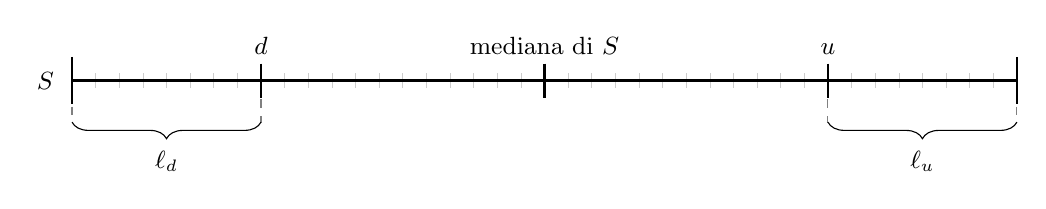
\begin{tikzpicture}[scale=1.2, every node/.style={font=\small}]

    \foreach \i in {1,2,...,39}
        \draw[gray!40, very thin] ({-5 + \i*(10/40)}, 0.08) -- ({-5 + \i*(10/40)}, -0.08);

    \foreach \x in {-3, 0, 3}
        \draw[thick] (\x, 0.18) -- (\x, -0.18);

    \node[above=6pt] at (-3,0) {$d$};
    \node[above=6pt] at (3,0) {$u$};
    \node[above=6pt] at (0,0) {mediana di $S$};

    \draw[gray, thin, dashed] (-5,-0.1) -- (-5,-0.45);
    \draw[gray, thin, dashed] (-3,-0.2) -- (-3,-0.45);
    \draw[gray, thin, dashed] (3,-0.2) -- (3,-0.45);
    \draw[gray, thin, dashed] (5,-0.1) -- (5,-0.45);

    % Graffa sinistra (da inizio a d)
    \draw[decorate, decoration={brace, mirror, raise=15pt, amplitude=6pt}]
        (-5,0) -- (-3,0)
        node[midway, below=22pt] {$\ell_d$};

    % Graffa destra (da u a fine)
    \draw[decorate, decoration={brace, mirror, raise=15pt, amplitude=6pt}]
        (3,0) -- (5,0)
        node[midway, below=22pt] {$\ell_u$};


    % Disegno dell'Array S
    \draw[thick] (-5,0) -- (5,0);
    \draw[thick] (-5,0.25) -- (-5,-0.25);
    \draw[thick] (5,0.25) -- (5,-0.25);
    \node[left=3pt] at (-5,0) {$S$};
    \end{tikzpicture}
\end{center}
